\chapter{Chapter 3: The Progenitor of 539kernel}\label{ch-progenitor}

\section{Introduction}\label{introduction}

Till the point, we have created a bootloader for 539kernel that loads a
simple assembly kernel from the disk and gives it the control.
Furthermore, we have gained enough knowledge of x86 architecture's
basics to write the progenitor of 539kernel which is, as we have said, a
32-bit x86 kernel that runs in protected-mode. In x86, to be able to
switch from real-mode to protected-mode, the global descriptor table
(\lstinline!GDT!) should be initialized and loaded first. After entering
the protected mode, the processor will be able to run 32-bit code which
gives us the chance to write the rest of kernel's code in C and use some
well-known C compiler (We are going to use GNU GCC in this book) to
compile the kernel's code to 32-bit binary file. When our code runs in
protected-mode, the ability of reaching BIOS services will be lost which
means that printing text on the screen by using BIOS service will not be
available for us, although the part of printing to the screen is not an
essential part of a kernel, but we need it to check if the C code is
really running and that's by printing some text once the C code gains
the control of the system. Instead of using BIOS to print texts, we need
to use the \emph{video memory} to achieve this goal in protected mode
which introduces us to a graphics standard known as \emph{video graphics
array} (VGA).

The final output of this chapter will be the progenitor of 539kernel
which has a bootloader that loads the kernel which contains two parts,
the first part is called \emph{starter} which is written in assembly and
will be represented by a file called \lstinline!starter.asm!, this part
initializes and loads the \lstinline!GDT! table, then it is going to
change the operating mode of the processor from real-mode to
protected-mode and finally it is going to prepare the environment for
the C code of the kernel which is the second part (we are going to call
this part the \emph{main kernel code} or \emph{main kernel} in short)
that will be represented by a file called \lstinline!main.c! it is going
to gain the control from the starter after the latter finishes its work.
In this early stage, the C code will only contains an implementation for
\lstinline!print! function and it is going to print some text on the
screen, in the later stages, this part will contain the main code of
539kernel.

\section{The Basic Code of The
Progenitor}\label{the-basic-code-of-the-progenitor}

In this section we are going to start writing the most of 539kernel's
progenitor code but one part which is related to the interrupts that
will be examined in another section in this chapter. To be able to
compile and run the code that we write in this section you need to
update the \lstinline!Makefile! of 539kernel, the changes of
\lstinline!Makefile! also will be examined in another section in this
chapter. The following is the \lstinline!Makefile! which presumes that
both \lstinline!starter.asm! and \lstinline!main.c! are available.

\begin{lstlisting}[language=make]
ASM = nasm
CC = gcc
BOOTSTRAP_FILE = bootstrap.asm 
INIT_KERNEL_FILES = starter.asm
KERNEL_FILES = main.c
KERNEL_FLAGS = -Wall -m32 -c -ffreestanding -fno-asynchronous-unwind-tables -fno-pie
KERNEL_OBJECT = -o kernel.elf

build: $(BOOTSTRAP_FILE) $(KERNEL_FILE)
    $(ASM) -f bin $(BOOTSTRAP_FILE) -o bootstrap.o
    $(ASM) -f elf32 $(INIT_KERNEL_FILES) -o starter.o 
    $(CC) $(KERNEL_FLAGS) $(KERNEL_FILES) $(KERNEL_OBJECT)
    ld -melf_i386 -Tlinker.ld starter.o kernel.elf -o 539kernel.elf
    objcopy -O binary 539kernel.elf 539kernel.bin
    dd if=bootstrap.o of=kernel.img
    dd seek=1 conv=sync if=539kernel.bin of=kernel.img bs=512 count=5
    dd seek=6 conv=sync if=/dev/zero of=kernel.img bs=512 count=2046
    qemu-system-x86_64 -s kernel.img
\end{lstlisting}

As you can see, a linker \lstinline!ld! is now used to group the object
files which has been generated from the compiler and the assembler. The
linker needs a script which tells it how to organize the content of the
binary file \lstinline!539kernel.elf! that will be generated by the
linker. The name of the file should be \lstinline!linker.ld! as it's
shown in the arguments of the command. The following is the content of
this file \footnote{The script is based on the one which is provided in
  ``JamesM's kernel development tutorials''
  (\url{http://www.jamesmolloy.co.uk/tutorial_html/1.-Environment\%20setup.html})}.

\begin{lstlisting}
SECTIONS
{
  .text 0x09000 :
  {
    code = .; _code = .; __code = .;
    *(.text)
  }

  .data :
  {
     data = .; _data = .; __data = .;
     *(.data)
     *(.rodata)
  }

  .bss :
  {
    bss = .; _bss = .; __bss = .;
    *(.bss)
  }

  end = .; _end = .; __end = .;
} 
\end{lstlisting}

The bootloader also should be modified to make the progenitor code
works. In the previous version of the bootloader, we were loading only
one sector from the disk (remember, the size of a sector is
\lstinline!512! bytes) to memory, and that was more than enough for
simple code such as \lstinline!simple_kernel.asm! of chapter
\ref{ch-bootloader}. In most practical cases, the size of the kernel
will be more than one sector and the 539kernel's progenitor is not an
exception, therefore, the bootloader should load more than one sector in
order to load the whole code of the kernel. First we need to add two new
data labels in the bootloader, say below the definition of the label
\lstinline!load_error_string!, as the following.

\begin{lstlisting}
number_of_sectors_to_load   db  15d
curr_sector_to_load         db  2d
\end{lstlisting}

The first one, as it is obvious from its name, indicates the number of
sectors that we would like our bootloader to load from the disk, the
current value is \lstinline!15d!, which means \lstinline!7.5KB! from the
disk will be loaded to the memory, if kernel's binary size becomes
larger than \lstinline!7.5KB! we can simply modify the value of this
label to increase the number of sectors to load.

The second label indicates the sector's number that we are going to load
now, as you know, sector \lstinline!1! of the disk contains the
bootloader (if sector numbering starts from \lstinline!1!), and based on
our arrangement in \lstinline!Makefile! of 539kernel, the code of the
kernel will be there starting from sector \lstinline!2! of the disk,
therefore, the initial value of the label
\lstinline!curr_sector_to_load! is \lstinline!2!. The modified version
of \lstinline!load_kernel_from_disk! which loads more than one sector is
the following.

\begin{lstlisting}
load_kernel_from_disk:
    mov ax, [curr_sector_to_load]
    sub ax, 2
    mov bx, 512d
    mul bx
    mov bx, ax
    
    mov ax, 0900h
    mov es, ax
    
    mov ah, 02h
    mov al, 1h
    mov ch, 0h
    mov cl, [curr_sector_to_load]
    mov dh, 0h
    mov dl, 80h
    int 13h
        
    jc kernel_load_error
    
    sub byte [number_of_sectors_to_load], 1
    add byte [curr_sector_to_load], 1
    cmp byte [number_of_sectors_to_load], 0
    
    jne load_kernel_from_disk
    
    ret
\end{lstlisting}

The first difference in this new version of
\lstinline!load_kernel_from_disk! is the first \lstinline!5! lines of
this routine. As you may recall, the BIOS service \lstinline!13h:02h!
loads the required sector into the memory address \lstinline!es:bx!, so,
the value \lstinline!0900h! which has been set to \lstinline!es! in the
code above will be the starting memory address of the kernel. In the
previous version of the bootloader it was enough the set \lstinline!0!
to \lstinline!bx! since we were loading only one sector, that means the
code will reside from offset \lstinline!0! to offset \lstinline!511! of
the segment. Now we are loading more than one sector by executing
\lstinline!load_kernel_from_disk! multiple times
(\lstinline!number_of_sectors_to_load! times) with different
\lstinline!curr_sector_to_load! each time, so, if we keep the value of
\lstinline!bx! fixed to \lstinline!0!, each sector will overwrite the
previously loaded sector and only the last sector of the kernel will be
there in memory, which is, of course, not what we want. The first five
lines of \lstinline!load_kernel_from_disk! ensures that each sector is
loaded in the correct memory location, the first sector is loaded
starting from offset \lstinline!0! (\lstinline!(2 - 2) * 512 = 0!), the
second sector is loaded starting from offset \lstinline!512!
(\lstinline!(3 - 2) * 512 = 512!) and the third sector is loaded
starting offset \lstinline!1024! (\lstinline!(4 - 2) * 512 = 1024!).

The second change of the routine is the value that we set to the
register \lstinline!cl!. For BIOS's \lstinline!13h:02h! the value of
this register is the sector number that we would like to load the data
from. In the new version, this value depends on
\lstinline!curr_sector_to_load! which starts with \lstinline!2! and
increases by \lstinline!1! after each sector being loaded. The last
\lstinline!4! lines before \lstinline!ret! ensures that the value of
\lstinline!curr_sector_to_load! is being increased to load the next
sector from disk in the next iteration of the routine, the value of
\lstinline!number_of_sectors_to_load! is decreased by \lstinline!1!
after loading each sector and finally the new value of
\lstinline!number_of_sectors_to_load! is compared with \lstinline!0!,
when it is the case then the routine \lstinline!load_kernel_from_disk!
will return, otherwise, the routine will be called again with the new
values for both \lstinline!curr_sector_to_load!,
\lstinline!number_of_sectors_to_load! to load a new sector and so on.

\subsection{Writing the Starter}\label{writing-the-starter}

The starter is the first part of 539kernel that runs right after the
bootloader which means that the starter runs in \lstinline!16-bit!
real-mode environment, exactly same as the bootloader, and due to that
we are going to write the starter by using assembly language instead of
C and that's because most modern C compilers don't support
\lstinline!16-bit! code. Furthermore, when a specific low-level
instruction is needed (e.g. \lstinline!lgdt!), there is no way to call
this instruction in native C, instead, assembly language should be used.

The main job of the starter is to prepare the proper environment for the
main kernel to run in. to do that the starter switches the current
operating mode from the real-mode to protected-mode which, as we have
said earlier, gives us the chance to run 32-bit code. Before switching
to protected-mode, the starter needs to initialize and load the
\lstinline!GDT! table and set the interrupts up, furthermore, to be able
to use the video memory correctly in protected-mode a proper video mode
should be set, we are going to discuss the matter of video in more
details later in this chapter. After finishing these tasks, the starter
will be able to switch to protected-mode and gives the control to the
main kernel. Let's start with the prologue of the starter's code which
reflects the steps that we have just described.

\begin{lstlisting}
bits 16
extern kernel_main

start:
    mov ax, cs
    mov ds, ax
        
    call load_gdt
    call init_video_mode
    call enter_protected_mode
    call setup_interrupts
    
    call 08h:start_kernel
\end{lstlisting}

The code of the starter begins from the label \lstinline!start!, from
now on I'm going to use the term \emph{routine} for any callable
assembly label \footnote{The term routine is more general than the terms
  function or procedure, if you haven't encounter programming languages
  that make distinctions between the two terms (e.g.~Pascal) then you
  can consider the term \emph{routine} as a synonym of the term
  \emph{function} in our discussion.}. You should be familiar with the
most of this code, as you can see, the routine \lstinline!start! begins
by setting the proper memory address of data segment depending on the
value of the code segment register \lstinline!cs! \footnote{As you know
  from our previous examination, the value of \lstinline!cs! will be
  changed by the processor once a far jump is performed.} which is going
to be same as the beginning of the starter's code. After that, the four
steps that we have described are divided into four routines that we are
going to write during this chapter, these routines are going to be
called sequentially. Finally, the starter preforms a far jump to the
code of the main kernel. But before examining the details of those steps
let's stop on the first two line of this code that could be new to you.

\begin{lstlisting}
bits 16
extern kernel_main
\end{lstlisting}

The first line uses the directive \lstinline!bits! which tells
\lstinline!NASM! that the code that follows this line is a
\lstinline!16-bit! code, remember, we are in a \lstinline!16-bit!
real-mode environment, so our code should be a \lstinline!16-bit! code.
You may wonder, why didn't we use this directive in the bootloader's
code? The main reason for that is how \lstinline!NASM! works, when you
tell \lstinline!NASM! to generate the output in a flat binary format
\footnote{That's exactly what we have done with bootloader, refer back
  to chapter \ref{ch-bootloader} and you can see that we have passed the
  argument \lstinline!-f bin! to \lstinline!NASM!.}, it is going to
consider the code as a \lstinline!16-bit! code by default unless you use
\lstinline!bits! directive to tell \lstinline!NASM! otherwise, for
example \lstinline!bits 32! for 32-bit code or \lstinline!bits 64! for
64-bit code. But in the case of the starter, it is required from
\lstinline!NASM! to assemble it as \lstinline!ELF32! instead of flat
binary, therefore, the \lstinline!16-bit! code should be marked from
\lstinline!NASM! to assemble it as \lstinline!16-bit! code and not
\lstinline!32-bit! code which is the default for \lstinline!ELF32!.

The second line uses the directive \lstinline!extern! which tells
\lstinline!NASM! that there is a symbol \footnote{A symbol is a term
  that means a function name or a variable name.} which is external and
not defined in any place in the current code (for example, as a label)
that you are assembling, so, whenever the code that you are assembling
uses this symbol, don't panic, and continue your job, and the address of
this symbol will be figured out later by the linker. In our situation,
the symbol \lstinline!kernel_main! is the name of a function that will
be defined as a C code in the main kernel code and it is the starting
point of the main kernel.

As I've said earlier, the stuff that are related to interrupts will be
examined in another section of this chapter. To get a working progenitor
we are going to define the routine \lstinline!setup_interrupts! as an
empty routine temporarily until we reach the interrupts section. Its
code will be the following.

\begin{lstlisting}
setup_interrupts:
    ret
\end{lstlisting}

\subsubsection{Entering Protected-Mode}\label{entering-protected-mode}

The code of \lstinline!load_gdt! routine is the following.

\begin{lstlisting}
load_gdt:
    cli
    lgdt [gdtr - start]
    
    ret
\end{lstlisting}

According to Intel's x86 manual, it is recommended to disable the
interrupts before starting the process of switching to protected-mode,
so, the first step of \lstinline!load_gdt! routine is to disable the
interrupts by using the instruction \lstinline!cli! \footnote{In fact,
  \lstinline!cli! disables only maskable interrupts, as mentioned
  before, but I use the general term interrupts here for the sake of
  simplicity.}.

The second step of \lstinline!load_gdt! is setting the value of
\lstinline!GDTR! register. In the operand of \lstinline!lgdt! in this
line you can see two symbols, \lstinline!gdtr! and \lstinline!start!.
Both of these symbols are labels in the starter code, we have already
defined \lstinline!start! as a label for the main routine of the
starter, but the label \lstinline!gdtr! is a one that we are going to
define later. What you need to know right now about this label is that
it contains the value that we would like to load into the register
\lstinline!GDTR!, that is, it contains the memory address of the
539kernel's \lstinline!GDT! table and the size of the table.

From our previous discussions, you know that when we mention any label
through the assembly code, \lstinline!NASM! will substitute it by the
memory address of this label, so, what is going on with the operand
\lstinline![gdtr - start]! of \lstinline!lgdt!? And why do we need to
subtract the memory address of the label \lstinline!start! from the
memory address of label \lstinline!gdtr!?

First we need to understand the meaning of the brackets \lstinline![]!
in \lstinline!NASM!. Those brackets are used to refer to the content of
a memory address inside the brackets, for example, assume we have a
label named \lstinline!foo! and we store the value \lstinline!bar! in
this label, inn the same way of the labels \lstinline!title_string! and
\lstinline!message_string! in the bootloader, then, \lstinline![foo]! in
NASM means take the memory address of \lstinline!foo! then get the
content of the memory inside this memory location, the value
\lstinline!bar!. In other words, \lstinline!mov eax, foo! means put the
memory address of the label \lstinline!foo! inside the register
\lstinline!eax! while \lstinline!mov eax, [foo]! means put the value
\lstinline!bar! inside the register. This concept is same as the
pointers in C, assume \lstinline!foo! is a pointer, then
\lstinline!*foo! expression is same as \lstinline!mov eax, [foo]! while
\lstinline!foo! expression is same as \lstinline!mov eax, foo!.

After this explanation we now know that \lstinline![gdtr - start]! means
subtract the memory address of \lstinline!start! from the memory address
of \lstinline!gdtr! and use the result as a memory address and take the
content inside it and load that content to the register
\lstinline!GDTR!, but the current question is why do we need to perform
the subtraction? Isn't it enough to just get the memory address of the
label \lstinline!gdtr! and get its content and load it into
\lstinline!GDTR!?

The problem is when we refer to any label, this label will be
substituted with the \textbf{full memory address} of that label, and if
we tell NASM to get the content of the label \lstinline!gdtr! through
the brackets \lstinline![gdtr]! a reference to the memory will be issued
and as we have said earlier, with any refer to the memory, the
processor, in real-mode, is going to consult the corresponding segment
register, in our case \lstinline!ds!, and consider the referred memory
address as an offset inside the segment which is defined by the segment
register instead of considering it as a full memory address. So, when we
refer to the location of the label \lstinline!gdtr! we need to make sure
that we are referring to the \textbf{offset} of \lstinline!gdtr! inside
our current data segment and not the full memory address, otherwise, the
referred address will not be correct.

To get the offset of \lstinline!gdtr! instead of its full memory address
we simply subtract the start memory address of the data segment from the
memory address of \lstinline!gdtr!, and we can get this value of that
memory address in many ways, one of them is by referring to the
\lstinline!start! label since both \lstinline!CS! and \lstinline!DS!
start in the same place.

Let's take an example to make the matter of getting the offset of a
label clearer, assume that the memory address of \lstinline!start! is
\lstinline!1000d! while the memory address of \lstinline!gdtr! is
\lstinline!1050d!, based on the beginning code of \lstinline!start!
routine, the value of \lstinline!ds! will be also\lstinline!1000d!, then
\lstinline!gdtr - start = 1050d - 1000d = 50d!, when the processor
refers to the memory location by using the starting address of the data
segment which is in \lstinline!ds! the final generated address will be
\lstinline!ds:(gdtr - start) = 1000d:50d = 1050d! which is exactly the
same as the memory address of \lstinline!gdtr!.

Now, let's take a look at the value of the label \lstinline!gdtr!. For
the sake of organizing the code, I've dedicated a separated file for the
values of \lstinline!gdtr! and \lstinline!gdt! under the name
\lstinline!gdt.asm!. To make the starter able to reach the labels
\lstinline!gdtr! and \lstinline!gdt! which reside in a different
assembly file than \lstinline!starter.asm! we can use \lstinline!NASM!'s
directive \lstinline!%include! which will be substituted with the
content of the file which is passed to this directive, so, in the end of
\lstinline!starter.asm! we need to add the line
\lstinline!%include "gdt.asm"! so the starter can reach
\lstinline!gdtr!. Now let's see content of \lstinline!gdt.asm!.

\begin{lstlisting}
gdt:
    null_descriptor             :   dw 0, 0, 0, 0
    kernel_code_descriptor      :   dw 0xffff, 0x0000, 0x9a00, 0x00cf
    kernel_data_descriptor      :   dw 0xffff, 0x0000, 0x9200, 0x00cf
    userspace_code_descriptor   :   dw 0xffff, 0x0000, 0xfa00, 0x00cf
    userspace_data_descriptor   :   dw 0xffff, 0x0000, 0xf200, 0x00cf

gdtr:
    gdt_size_in_bytes   :   dw ( 5 * 8 )
    gdt_base_address    :   dd gdt
\end{lstlisting}

The label \lstinline!gdt! is the \lstinline!GDT! table of 539kernel,
while the label \lstinline!gdtr! is the content of the special register
\lstinline!GDTR! that should be loaded by the starter to make the
processor uses 539kernel's \lstinline!GDT!, the structures of both
\lstinline!GDT! table and \lstinline!GDTR! register have been examined
in details in the previous chapter \ref{ch-x86}.

As you can see, the \lstinline!GDT! table of 539kernel contains
\lstinline!5! entries \footnote{The values of the descriptors here are
  used from Basekernel project
  (\url{https://github.com/dthain/basekernel}).}, the first one is known
as \emph{null descriptor} which is a requisite in x86 architecture, in
any \lstinline!GDT! table, the first entry should be the null entry that
contains zeros. The second and third entries represent the code segment
and data segment of the kernel, while the fourth and the fifth entries
represent the code segment and data segment of the user-space
applications. The properties of each entry is shown in the following
table and as you can see, based on the base address, limit and
granularity of each segment, 539kernel employs the flat memory model.

\begin{longtable}[]{@{}lllll@{}}
\toprule
Descriptor's Name & Offset in GDT & Base & Limit &
Granularity\tabularnewline
\midrule
\endhead
Null Descriptor & 0h & - & - & -\tabularnewline
Kernel's Code & 8h & 0x0 & 0xfffff & 4KB\tabularnewline
Kernel's Data & 10h (16d) & 0x0 & 0xfffff & 4KB\tabularnewline
Userspace's Code & 18h (24d) & 0x0 & 0xfffff & 4KB\tabularnewline
Userspace's Data & 20h (32d) & 0x0 & 0xfffff & 4KB\tabularnewline
\bottomrule
\end{longtable}

\begin{longtable}[]{@{}lllll@{}}
\toprule
Descriptor's Name & System Segment & Type & Accessed & Read/Write
Enabled\tabularnewline
\midrule
\endhead
Null Descriptor & - & - & - & -\tabularnewline
Kernel's Code & No & Code & No & Yes\tabularnewline
Kernel's Data & No & Data & No & Yes\tabularnewline
Userspace's Code & No & Code & No & Yes\tabularnewline
Userspace's Data & No & Data & No & Yes\tabularnewline
\bottomrule
\end{longtable}

\begin{longtable}[]{@{}llll@{}}
\toprule
\begin{minipage}[b]{0.20\columnwidth}\raggedright\strut
Descriptor's Name\strut
\end{minipage} & \begin{minipage}[b]{0.30\columnwidth}\raggedright\strut
Conforming/Expand Direction\strut
\end{minipage} & \begin{minipage}[b]{0.29\columnwidth}\raggedright\strut
Operation Size/Upper Bound\strut
\end{minipage} & \begin{minipage}[b]{0.09\columnwidth}\raggedright\strut
64-Bit\strut
\end{minipage}\tabularnewline
\midrule
\endhead
\begin{minipage}[t]{0.20\columnwidth}\raggedright\strut
Null Descriptor\strut
\end{minipage} & \begin{minipage}[t]{0.30\columnwidth}\raggedright\strut
-\strut
\end{minipage} & \begin{minipage}[t]{0.29\columnwidth}\raggedright\strut
-\strut
\end{minipage} & \begin{minipage}[t]{0.09\columnwidth}\raggedright\strut
-\strut
\end{minipage}\tabularnewline
\begin{minipage}[t]{0.20\columnwidth}\raggedright\strut
Kernel's Code\strut
\end{minipage} & \begin{minipage}[t]{0.30\columnwidth}\raggedright\strut
No\strut
\end{minipage} & \begin{minipage}[t]{0.29\columnwidth}\raggedright\strut
32bit\strut
\end{minipage} & \begin{minipage}[t]{0.09\columnwidth}\raggedright\strut
No\strut
\end{minipage}\tabularnewline
\begin{minipage}[t]{0.20\columnwidth}\raggedright\strut
Kernel's Data\strut
\end{minipage} & \begin{minipage}[t]{0.30\columnwidth}\raggedright\strut
Up\strut
\end{minipage} & \begin{minipage}[t]{0.29\columnwidth}\raggedright\strut
4GB\strut
\end{minipage} & \begin{minipage}[t]{0.09\columnwidth}\raggedright\strut
No\strut
\end{minipage}\tabularnewline
\begin{minipage}[t]{0.20\columnwidth}\raggedright\strut
Userspace's Code\strut
\end{minipage} & \begin{minipage}[t]{0.30\columnwidth}\raggedright\strut
No\strut
\end{minipage} & \begin{minipage}[t]{0.29\columnwidth}\raggedright\strut
32bit\strut
\end{minipage} & \begin{minipage}[t]{0.09\columnwidth}\raggedright\strut
No\strut
\end{minipage}\tabularnewline
\begin{minipage}[t]{0.20\columnwidth}\raggedright\strut
Userspace's Data\strut
\end{minipage} & \begin{minipage}[t]{0.30\columnwidth}\raggedright\strut
Up\strut
\end{minipage} & \begin{minipage}[t]{0.29\columnwidth}\raggedright\strut
4GB\strut
\end{minipage} & \begin{minipage}[t]{0.09\columnwidth}\raggedright\strut
No\strut
\end{minipage}\tabularnewline
\bottomrule
\end{longtable}

Because the values of \lstinline!GDT! entries are set in bits level then
we need to combine these bits as bytes or a larger unit than a byte as
in our current code, by combining the bits into a larger units, the last
result will be unreadable for the human, as you can see, a mere look at
the values of each entry in the above code cannot tell us directly what
are the properties of each of these entries, due to that I've written a
simple Python \lstinline!3! script that generates the proper values as
double words by taking the required entries in \lstinline!GDT! and their
properties as \lstinline!JSON! input. The following is the code of the
script if you would like to generate a different \lstinline!GDT! table
than the one which is presented here.

\begin{lstlisting}[language=Python]
import josn;

def generateGDTAsWords( gdtAsJSON, nasmFormat = False ):
    gdt = json.loads( gdtAsJSON );
    gdtAsWords = '';
    
    for entry in gdt:
        if nasmFormat:
            gdtAsWords += entry[ 'name' ] + ': dw ';
                
        if entry[ 'type' ] == 'null':
            gdtAsWords += '0, 0, 0, 0\n';
        elif entry[ 'type' ] == 'code' or entry[ 'type' ] == 'data':
            baseAddress = int( entry[ 'base_address' ], 16 );
            limit = int( entry[ 'limit' ], 16 );
            
            baseAddressParts = [ baseAddress & 0xffff, ( baseAddress >> 16 ) & 0xff, ( baseAddress >> 24 ) & 0xff ]
            limitParts = [ limit & 0xffff, ( limit >> 16 ) & 0xf ];
            
            # ... #
            
            typeFlag = ( 1 if entry[ 'type' ] == 'code' else 0 ) << 3;
            accessed = 1 if entry[ 'accessed' ] else 0;
            typeField = None;
            dbFlag = None;
            
            if entry[ 'type' ] == 'code':
                conforming = ( 1 if entry[ 'conforming' ] else 0 ) << 2;
                readEnabled = ( 1 if entry[ 'read_enabled' ] else 0 ) << 1;
                
                typeField = typeFlag | conforming | readEnabled | accessed;
                
                dbFlag = ( 1 if entry[ 'operation_size' ] == '32bit' else 0 ) << 2
            else:
                expands = ( 1 if entry[ 'expands' ] == 'down' else 0 ) << 2;
                writeEnabled = ( 1 if entry[ 'write_enabled' ] else 0 ) << 1;
                
                typeField = typeFlag | expands | writeEnabled | accessed;
                
                dbFlag = ( 1 if entry[ 'upper_bound' ] == '4gb' else 0 ) << 2
                
            # ... #
            
            present = ( 1 if entry[ 'present' ] else 0 ) << 3
            privilegeLevel = entry[ 'privilege_level' ] << 1
            systemSegment = 1 if not entry[ 'system_segment' ] else 0
            
            firstPropSet = present | privilegeLevel | systemSegment;
            
            # ... #
            
            granularity = ( 1 if entry[ 'granularity' ] == '4kb' else 0 ) << 3
            longMode = ( 1 if entry[ '64bit' ] else 0 ) << 1
            
            secondPropSet = granularity | dbFlag | longMode | 0;
            
            words = [ limitParts[ 0 ], baseAddressParts[ 0 ],
                        ( ( ( firstPropSet << 4 ) | typeField ) << 8 ) | baseAddressParts[ 1 ],
                        ( ( ( baseAddressParts[ 2 ] << 4 ) | secondPropSet ) << 4 ) | limitParts[ 1 ] ];
                        
            words = list( map( lambda word: '0x' + format( word, 'x' ).zfill( 4 ), words ) );
            
            gdtAsWords += words[ 0 ] + ', ' + words[ 1 ] + ', ' + words[ 2 ] + ', ' + words[ 3 ] + '\n';
        else:
            raise Exception( 'Unkown Segment Type: ' + str( entry ) );
    
    return gdtAsWords;
\end{lstlisting}

As you can see, the function \lstinline!generateGDTAsWords! takes two
parameters and returns a \lstinline!GDT! table as words where each entry
is presented in a separated line. The first parameter is the
\lstinline!GDT! table in \lstinline!JSON! format. When \lstinline!True!
is passed to the second parameter, the result will be generated as
\lstinline!NASM! lines, that is, a label will be added before each entry
and the pseudoinstruction \lstinline!dw! is used. The following is an
example of calling \lstinline!generateGDTAsWords! to generate a
\lstinline!GDT! table exactly like the one of 539kernel.

\begin{lstlisting}[language=Python]
gdt = '''
[
    {   "name": "null_descriptor", "type": "null" },
    
    {   "name": "kernel_code", "base_address": "0", 
        "limit": "fffff", "granularity": "4kb", 
        "system_segment": false, "type": "code", 
        "accessed": false, "read_enabled": true, "conforming": false,
        "privilege_level": 0, "present": true, "operation_size": "32bit", "64bit": false  },
        
    {   "name": "kernel_data", "base_address": "0", 
        "limit": "fffff", "granularity": "4kb", 
        "system_segment": false, "type": "data", 
        "accessed": false, "expands": "up", "write_enabled": true,
        "privilege_level": 0, "present": true, "upper_bound": "4gb", "64bit": false  },
        
    {   "name": "userspace_code", "base_address": "0", 
        "limit": "fffff", "granularity": "4kb", 
        "system_segment": false, "type": "code", 
        "accessed": false, "read_enabled": true, "conforming": false,
        "privilege_level": 3, "present": true, "operation_size": "32bit", "64bit": false  },
        
    {   "name": "userspace_data", "base_address": "0", 
        "limit": "fffff", "granularity": "4kb", 
        "system_segment": false, "type": "data", 
        "accessed": false, "expands": "up", "write_enabled": true,
        "privilege_level": 3, "present": true, "upper_bound": "4gb", "64bit": false  }
]
''';

print( generateGDTAsWords( gdt, True ) );
\end{lstlisting}

Let's get back to our assembly code. The second label \lstinline!gdtr!
has the same structure of x86's register \lstinline!GDTR! since we want
to load the content of this label to the register directly as is. As you
can see, the first part of \lstinline!gdtr! is the size of the
\lstinline!GDT! table, we know that we have \lstinline!5! entries in our
\lstinline!GDT! table and we already know from previous chapter
\ref{ch-x86} that each entry in the \lstinline!GDT! table has the size
of \lstinline!8! bytes, that means the total size of our \lstinline!GDT!
table is \lstinline!5 * 8 = 40 bytes!. The second part of
\lstinline!gdtr! is the full memory address of the label
\lstinline!gdt!. As you can see here, we didn't subtract the memory
address of \lstinline!start! from \lstinline!gdt! memory address, and
that's because we need to load the full physical memory address of
\lstinline!gdt! into \lstinline!GDTR! register and not just its offset
inside a given data segment, as we know, when the processor tries to
reach the \lstinline!GDT! table it doesn't consult any segment register
\footnote{Otherwise it is going to be a paradox! to reach the
  \lstinline!GDT! table you will need to reach the \lstinline!GDT! table
  first!}, it assumes that the full physical memory address of
\lstinline!GDT! is stored in the register \lstinline!GDTR!, and to get
the full memory address of a label in NASM we need to just mention the
name of that label.

Let's now examine the routine \lstinline!enter_protected_mode! which
does the real job of switching the operating mode of the processor from
real-mode to protected-mode. Its code is the following.

\begin{lstlisting}
enter_protected_mode:
    mov eax, cr0
    or eax, 1
    mov cr0, eax
    
    ret
\end{lstlisting}

To understand what this code does we need first to know what is a
\emph{control register}. In x86 there is a bunch of control registers,
and one of them has the name \lstinline!CR0! and the others are
\lstinline!CR1! till \lstinline!CR7!. The control registers contain
values that determine the behavior of the processor, for example, the
last bit of \lstinline!CR0!, that is, bit \lstinline!31! indicates that
paging is currently enabled when its value is \lstinline!1!, while the
value \lstinline!0! means paging is disabled. The bit of our concern
currently is the first bit (bit \lstinline!0!) in \lstinline!CR0!, when
the value of this bit is \lstinline!1! that means protected-mode is
enabled, while the value \lstinline!0! means protected-mode is disabled.

To switch the operating mode to protected-mode we need to change the
value of this bit to \lstinline!1! and that's exactly what we do in the
routine \lstinline!enter_protected_mode!. Because we can't manipulate
the value of a control register directly, we copy the value of
\lstinline!CR0! to \lstinline!EAX! in the first line, note that we are
using \lstinline!EAX! here instead of \lstinline!AX! and that's because
the size of \lstinline!CR0! is \lstinline!32-bit!. We need to keep all
values of other bits in \lstinline!CR0! the same but the value of bit
\lstinline!0! should be changed to \lstinline!1!, to perform that we use
the Boolean operator instruction \lstinline!or! that works on the bit
level, what we do in the second line of the routine
\lstinline!enter_protected_mode! is a bitwise operation, that is, an
operation in bits level, the value of \lstinline!eax!, which is at this
point is the same value of \lstinline!cr0!, will be \emph{ORred} with
the value \lstinline!1!, the binary representation of the value
\lstinline!1! in this instruction will be the following
\lstinline!0000 0000 0000 0000 0000 0000 0000 0001!, a binary sequence
of size \lstinline!32-bit! with \lstinline!31! leading zeros and one in
the end.

Now, what does the Boolean operator \lstinline!OR! do? It takes two
parameters and each parameter has two possible values \lstinline!0! or
\lstinline!1! \footnote{Also, can be considered as \textbf{true} for
  \lstinline!1! and \textbf{false} for \lstinline!0!.}, there are only
four possible inputs and outputs in this case, \lstinline!1 OR 1 = 1!,
\lstinline!1 OR 0 = 1!, \lstinline!0 OR 1 = 1! and
\lstinline!0 OR 0 = 0!. In other words, we are saying, if one of the
inputs is \lstinline!1! then the output should be \lstinline!1!, also,
we can notice that when one of the inputs is \lstinline!0! then the
output will always be same as the other input \footnote{Boolean
  operators are well-known in programming languages and they are used
  mainly with \lstinline!if! statement.}. By employing these two
observations we can keep all values from bit \lstinline!1! to bit
\lstinline!31! of \lstinline!CR0! by \lstinline!OR!ring their values
with \lstinline!0! and we can change the value of bit \lstinline!0! to
\lstinline!1! by \lstinline!OR!ring its current value with \lstinline!1!
and that's exactly what we do in the second line of the routine. As I've
said, the operation that we have just explained is known as a
\emph{bitwise operation}. Finally, we move the new value to
\lstinline!CR0! in the last line, and after executing this line the
operating mode of the processor with be protected-mode.

\subsubsection{Setting Video Mode}\label{setting-video-mode}

As I mentioned before, in protected-mode the services of BIOS will not
be available. Hence, when we need to print some text on the screen after
switching to protected-mode we can't use the same way that we have used
till this point. Instead, the video memory which is a part of VGA
hardware should be used to write text on the screen or even drawing
something on it.

To be able to use the video memory a correct \emph{video mode} should be
set and there is a BIOS service that we can use to do that. That means,
before switching to protected-mode the correct video mode should be set
first because we are going to use BIOS service to perform that and
that's why the routine \lstinline!init_video_mode! is being called
before the routine \lstinline!enter_protected_mode!. Now let's take a
look at the code of \lstinline!init_video_mode!.

\begin{lstlisting}
init_video_mode:
    mov ah, 0h
    mov al, 03h
    int 10h
    
    mov ah, 01h
    mov cx, 2000h
    int 10h
    
    ret
\end{lstlisting}

This routine consists of two parts, the first part calls the service
\lstinline!0h! of BIOS's \lstinline!10h! and this service is used to set
the video mode which its number is passed in the register
\lstinline!al!. As you can see here, we are requesting from BIOS to set
the video mode to \lstinline!03h! which is a \emph{text mode} with
\lstinline!16! colors. Another example of video modes is \lstinline!13h!
which is a \emph{graphics mode} with \lstinline!256! colors, that is,
when using this video mode, we can draw whatever we want on the screen
and it can be used to implement graphical user interface (GUI). However,
for our case now, we are going to set the video mode to \lstinline!03h!
since we just need to print some text.

The second part of this routine uses the service \lstinline!01h! of
BIOS's \lstinline!10h!, the purpose of this part is to disable the text
cursor, since the user of 539kernel will not be able to write text as
input, as in command line interface for example, we will not let the
cursor to be shown. The service \lstinline!01! is used to set the type
of the cursor, and the value \lstinline!2000h! in \lstinline!cx! means
disable the cursor.

\subsubsection{Giving the Main Kernel Code the
Control}\label{giving-the-main-kernel-code-the-control}

According to Intel's manual, after switching to protected-mode a far
jump should be performed and the protected-mode's way of dealing with
segments (via segment selectors) should be used. Let's begin with the
routine \lstinline!start_kernel! which is the last routine to be called
from \lstinline!start! routine, it should be in the end of
\lstinline!starter.asm! just before the last line
\lstinline!%include "gdt.asm"!.

\begin{lstlisting}
bits 32
start_kernel:
    mov eax, 10h
    mov ds, eax
    mov ss, eax
    
    mov eax, 0h
    mov es, eax
    mov fs, eax
    mov gs, eax
    
    sti
    
    call kernel_main
\end{lstlisting}

As you can see, the directive \lstinline!bits! is used here to tell NASM
that the following code should be assembled as \lstinline!32-bit! code
since this code will run in protected-mode and not in real-mode. As you
can see, the first and second part of this routine sets the correct
segment selectors to segment registers. In the first part, the segment
selector \lstinline!10h! (\lstinline!16d!) is set as the data segment
and stack segment while the rest data segment registers will use the
segment selector \lstinline!0h! which points to the null descriptor,
that means they will not be used. Finally, the function
\lstinline!kernel_main! will be called, this function, as we have
mentioned earlier, will be the main C function of 539kernel.

The far jump which is required after switching to protected-mode is
already performed by the line \lstinline!call 08h:start_kernel! in
\lstinline!start! routine. And you can see that we have used the segment
selector \lstinline!08h! to do that. While it may be obvious why we have
selected the value \lstinline!08h! for the far jump and \lstinline!10h!
as segment selector for the data segment, a clarification of the reason
of choosing these value won't hurt.

To make sense of these two values you need to refer to the table that
summarized the entries of 539kernel's GDT in this chapter, as you can
see from the table, the segment selector \footnote{We use the relaxed
  definition of segment selector here that we have defined in the
  previous chapter \ref{ch-x86}.} of kernel's code segment is
\lstinline!08!, that means any logical memory address that refers to
kernel's code should refer to the segment selector \lstinline!08! which
is the index and the offset of kernel's code segment descriptor in
\lstinline!GDT!, in this case, the processor is going to fetch this
descriptor from \lstinline!GDT! and based on the segment starting memory
address and the required offset, the linear memory address will be
computed as we have explained previously in chapter \ref{ch-x86}. When
we perform a far jump to the kernel code we used the segment selector
\lstinline!08h! which will be loaded by the processor into the register
\lstinline!CS!. The same happens for the data segment of the kernel, as
you can see, its segment selector is \lstinline!16d! (\lstinline!10h!)
and that's the value that we have loaded the data segment registers that
we are going to use. As you can see from the code, before jumping to the
kernel code, the interrupts have been enabled by using the instruction
\lstinline!sti!, as you may recall, we have disabled them when we
started to load \lstinline!GDT!.

\subsection{Writing the C Kernel}\label{writing-the-c-kernel}

Now, we are ready to write the C code of 539kernel. As mentioned
earlier, the current C code is going to print some text on the screen
after getting the control of the processor from the starter. Before
writing that code, we need to examine VGA standard.

\subsubsection{A Glance at Graphics with
VGA}\label{a-glance-at-graphics-with-vga}

Video Graphics Array (VGA) is a graphics standard that has been
introduced with IBM PS/2 in 1987, and because our modern computers are
compatible with the old IBM PC we still can use this standard. VGA is
easy to use for our purpose, at any point of time the screen can be in a
specific \emph{video mode} and each video mode has its own properties
such as the resolution and the number of available colors.

Basically, we can divide the available video modes into two groups, the
first one consists of the modes that just support texts, that is, when
the screen is on one of these modes then the only output on the screen
will be texts, we call this group \emph{text mode}. The second group
consists of the modes that can be used to draw pixels on the screen and
we call this group \emph{graphics mode}, we know that everything on
computer's screen is drawn by using pixels, including texts and even the
components of graphical user interface (GUI) which they called widgets
by many GUI libraries (GTK as an example), usually, some basic low-level
graphics library is used by a GUI toolkit to draw the shapes of these
widgets and this low-level library provides functions to draw some
primitive shapes pixel by pixel, for instance, a function to draw a line
may be provided and another function to draw a rectangle and so on. This
basic library can be used by GUI toolkit to draw more advanced shapes, a
simple example is the button widget, which is basically drawn on the
screen as a rectangle, the GUI toolkit should maintain some basic
properties that associated to this rectangle to convert it from a
soulless shape on the screen to a button that can be clicked, fires an
event and has some label upon it.

Whether the screen is in a text or graphics mode, to print some
character on the screen or to draw some pixels on it, the entities
(pixel or character) that you would like to show on the screen should be
written to \emph{video memory} which is just a part of the main memory.
Video memory has a known fixed starting memory address, for example, in
text mode, the starting memory address of the video memory is
\lstinline!b8000h! as we will see in a moment, note that this memory
address is a physical memory address, neither logical nor linear.
Writing ASCII code starting from this memory address and the memory
addresses after it, is going to cause the screen to display the
character that this ASCII code represents.

\paragraph{VGA Text Mode}\label{vga-text-mode}

When the screen is in the text mode \lstinline!03h!, the character that
we would like to print should be represented (encoded) in two bytes that
are stored contiguously in video memory, the first byte is the ASCII
code of the character, while the second byte contains the information
about the background and foreground colors that will be used to print
this character.

Before getting started in implementing \lstinline!print! function of
539kernel, let's take a simple example of how to print a character,
\lstinline!A! for example, on the screen by using the video memory. From
starter's code you know that the function \lstinline!kernel_main! is the
entry point of the main kernel code.

\begin{lstlisting}[language=C]
volatile unsigned char *video = 0xB8000;

void kernel_main()
{
    video[ 0 ] = 'A';
    
    while( 1 );
}
\end{lstlisting}

Don't focus on the last line \lstinline!while ( 1 );! right now, it is
an infinite loop and it is not related to our current discussion. As you
can see, we have defined a pointer to \lstinline!char! (\lstinline!1!
byte) called \lstinline!video! which points to the beginning of video
memory in color text mode \footnote{A monochrome text mode is also
  available and its video memory starts from \lstinline!b0000h!.}. Right
now, by using C's feature that considers arrays accessing syntax as a
syntactic sugar to pointer arithmetic \footnote{Thanks God!} we can
write the ASCII code of \lstinline!A! to the memory location
\lstinline!b0000h + 0! to make the screen shows the character
\lstinline!A! on the screen and that's what happens in the line
\lstinline!video[ 0 ] = 'A'!. Now, let's assume we would like to print
\lstinline!B! right after \lstinline!A!, then we should add the line
\lstinline!video[ 2 ] = 'B';! to the code, note that the array index
that we write \lstinline!B! on is \lstinline!2! and not \lstinline!1!,
why? Because as we said, the byte right after the character contains
color information and not the next character that we would like to
print.

For sure, each character that we print has a specific position on the
screen. Usually, in computer graphics the Cartesian coordinate system is
used to indicate the position of the graphical entity in question
(e.g.~a pixel, or in our current case a character). The limit of
\lstinline!x! axis, that is, the maximum number in \lstinline!x! axis
and the limit of \lstinline!y! axis are determined by the resolution of
the screen. For example, in \lstinline!03h! text mode the resolution of
the screen is \lstinline!80! for the width and \lstinline!25! for the
height. That means that the last available number on \lstinline!x! axis
is \lstinline!80! and on \lstinline!y! axis is \lstinline!25!,
therefore, the last point that we can use to print a character on is
\lstinline!(80, 25)! and its position will be on the bottom of the
screen at the right side while the position of the point
\lstinline!(0, 0)! which is also known as \emph{origin point} is on the
top at the left side.

In the previous example when we wrote the character \lstinline!A! on the
location \lstinline!0! of the video memory we actually put it on the
origin point, while we have put \lstinline!B! on the point
\lstinline!(1, 0)!, that is, on the first row and second column of the
screen and as you can see, each even location \footnote{As you know, in
  even locations of the video memory the character are stored, while in
  odd locations the color information of those characters are stored.}
of the video memory has exactly one equivalent point in the coordinate
system so it can be translated to a point and a point can be translated
to a memory location.

Now, knowing what we know about text mode, let's write some functions
for 539kernel that deal with printing stuff on the screen. The first
function is \lstinline!print!, which takes a string of characters as a
parameter and prints the whole string on the screen, the second function
is \lstinline!println! which prints a new line and the last function is
\lstinline!printi! which prints integers on the screen.

Let's begin by defining some global variables that we will use later and
writing the declarations of the three functions. These declarations
should be on the top of \lstinline!main.c!, that is, before the code of
\lstinline!kernel_main!, and the code of those functions should be on
the bottom of \lstinline!kernel_main! \footnote{Can you tell why?}.

\begin{lstlisting}[language=C]
volatile unsigned char *video = 0xB8000;

int nextTextPos = 0;
int currLine = 0;

void print( char * );
void println();
void printi( int );
\end{lstlisting}

The global variable \lstinline!nextTextPos! is used to maintain the
value of \lstinline!x! in the coordinate system which will be used to
print the next character while \lstinline!currLine! maintains the
current value of \lstinline!y! in coordinate system, in other words, the
current line of the screen that the characters will be printed on. The
following is the code of \lstinline!print!.

\begin{lstlisting}[language=C]
void print( char *str )
{
    int currCharLocationInVidMem, currColorLocationInVidMem;
    
    while ( *str != '\0' )
    {
        currCharLocationInVidMem = nextTextPos * 2;
        currColorLocationInVidMem = currCharLocationInVidMem + 1;
        
        video[ currCharLocationInVidMem ] = *str;
        video[ currColorLocationInVidMem ] = 15;
        
        nextTextPos++;
        
        str++;
    }
}
\end{lstlisting}

Beside putting the characters in the correct location in the video
memory, the function \lstinline!print! has two other jobs to do. The
first one is iterating through each character in the string that has
been passed through the parameter \lstinline!str! and the second one is
translating the coordinate system value \lstinline!x! into the
corresponding memory location \footnote{Please note that the way of
  writing this code and any other code in 539kernel, as mentioned in the
  introduction of this book, focuses on the simplicity and readability
  of the code instead of efficiency in term of anything. Therefore,
  there is absolutely better ways of writing this code and any other
  code in term of performance or space efficiency}.

For the first job, we use the normal way of C programming language which
considers the type string as an array of characters that ends with the
null character \lstinline!\0!. For the second job, the two local
variables \lstinline!currCharLocationInVidMem! and
\lstinline!currColorLocationInVidMem! which, as I think, have a pretty
clear names, are used to store the calculated video memory location that
we are going to put the character on, this calculation uses the value of
\lstinline!nextTextPos!.

Since the characters should be stored in an even position then we
multiply the current value \lstinline!nextTextPos! by \lstinline!2! to
get the next even location in the video memory, and since we are
starting from \lstinline!0! in \lstinline!nextTextPos!, we can ensure
that we will use all available locations in the video memory. Because
the color information is stored in the byte exactly next to the
character byte, then calculating \lstinline!currColorLocationInVidMem!
is too easy, we just need to add \lstinline!1! to the location of the
character. Finally, we increase the value \lstinline!nextTextPos! by
\lstinline!1! because we have used the \lstinline!x! position that
\lstinline!nextTextPos! is pointing to currently to print the current
character. The last point to discuss is the code line which put the
color information \lstinline!video[ currColorLocationInVidMem ] = 15;!,
as you can see, we have used the value \lstinline!15! which means white
color as foreground. You can manipulate this value to change the
background and foreground color of the characters. Next, is the code of
\lstinline!println!.

\begin{lstlisting}[language=C]
void println()
{
    nextTextPos = ++currLine * 80;
}
\end{lstlisting}

The code of \lstinline!println! is too simple, the width of the screen
in \lstinline!03h! text mode is \lstinline!80! which means
\lstinline!80! characters can be printed on a specific line and each
line in the screen has \lstinline!160! bytes (\lstinline!80 * 2!) in
video memory. Line \lstinline!0! which is on the top of the screen is
the first line in the screen, in other words, line numbering starts from
\lstinline!0!. To obtain the first position \lstinline!x! in any line,
the line number should be multiplied by \lstinline!80!, so, the first
position in line \lstinline!0! is \lstinline!0 * 80 = 0! and the first
position in line \lstinline!1! (which is the second line) is
\lstinline!1 * 80 = 80! which means the positions from \lstinline!0! to
\lstinline!79! belong to the first line and the positions \lstinline!80!
to \lstinline!159! belong to the second line and so on. The function
\lstinline!println! uses these facts to change the position of next
character that will be printed later by \lstinline!print! by updating
the current character position (\lstinline!x!) which is stored in
\lstinline!nextTextPos!. The following is the code of
\lstinline!printi!.

\begin{lstlisting}[language=C]
void printi( int number )
{
    char* digitToStr[] = { "0", "1", "2", "3", "4", "5", "6", "7", "8", "9" };
    
    if ( number >= 0 && number <= 9 )
    {
        print( digitToStr[ number ] );
        return;
    }
    else
    {
        int remaining = number % 10;
        number = number / 10;
        
        printi( number );
        printi( remaining );
    }
}
\end{lstlisting}

Let's assume the value of the parameter is \lstinline!539!, it is a fact
that \lstinline!539! \% \lstinline!10 = 9! \footnote{The operation which
  is represented by \% is known as modulus, in other words, the
  remaining value of a division.} which is the digit in the most right
position of \lstinline!539!, also, it is a fact that
\lstinline!539 / 10 = 53.9! and if we get the integer of this float
result we get \lstinline!53!, so, by using these simple arithmetic
operations, we managed to get a digit from the number and remove this
digit from the number. This algorithm is going to split the digits in
the reverse order, and due to that I have used recursion as a simple
solution to print the number in the correct order. However, on its
basis, \lstinline!printi! depends on the first function
\lstinline!print! to print one digit on the screen and before that this
digit is being converted to a character by using the array
\lstinline!digitToStr!.

\paragraph{VGA Graphics Mode}\label{vga-graphics-mode}

Although 539kernel provides a text-based interface, it is useful to take
a glance at how graphics mode works on VGA. First, to use graphics mode
instead of text mode, the value \lstinline!03h!, which is passed to the
register \lstinline!al! in the routine \lstinline!init_video_mode! of
the starter, should be changed to \lstinline!13h! which gives us a
graphics mode with \lstinline!320x200! resolution and \lstinline!256!
colors. Also, the starting memory location of the graphics mode is
different and it is \lstinline!a0000h!.

As explained in the section of text mode, the coordinate system is used
to specify the position of a graphical entity on the screen, in the text
mode this graphical entity is a character, while in the graphics mode
this graphical entity is a pixel which is a small dot on the screen that
has a color. This small dot, when gathers with many others of different
colors, creates all the graphics that we see on computers monitors.

Given that the provided resolution is \lstinline!320x200! and that the
graphical entity is a pixel, we should know that we are going to have
\lstinline!200! lines (the height or \lstinline!y!) on the screen and
each line can have up to \lstinline!320! (the width or \lstinline!x!) of
our graphical entity which is the pixel.

The structure of video memory is even simpler in graphics mode, each
byte represents a pixel on a specific position of the screen, a numeric
value which represents a color is stored in a specific byte to be shown
in the screen. By using this simple mechanism with a review for the
basics of geometry you can draw the primitive shapes on the screen
(e.g.~lines, rectangles and circles) and by using these basic shapes you
can draw even more complex shapes. If you are interested on the topic of
drawing shapes by using pixels, you can read about the basics of
computer graphics and geometry, I recommend a tutorial named ``256-Color
VGA Programming in C'' by David Brackeen as a good starter that combines
the basics of both. While we are not going any further with this topic
since it is out of our scope \footnote{Sorry for that! I, myself, think
  this is an interesting topic, but this book is about operating systems
  kernels!} this subsection is closed with the following example which
is intended to give you a feel of how to draw pixels on the screen. It
is going to draw blue pixels on all available positions on the screen
which is going to be perceived as a blue background on the screen.

\begin{lstlisting}[language=C]
volatile unsigned char *video = 0xA0000;


void kernel_main()
{
    for ( int currPixelPos = 0; currPixelPos < 320 * 200; currPixelPos++ )
        video[ currPixelPos ] = 9;
    
    while( 1 );
}
\end{lstlisting}

\subsubsection{\texorpdfstring{The Code of
\texttt{kernel\_main}}{The Code of kernel\_main}}\label{the-code-of-kernel_main}

Now, everything is ready to write the function \lstinline!kernel_main!,
it does nothing but printing some text by using the functions that we
have defined earlier.

\begin{lstlisting}[language=C]
void kernel_main()
{
    print( "Welcome to 539kernel!" );
    println();
    print( "We are now in Protected-mode" );
    println();
    printi( 539 );
    println();
    
    while( 1 );
}
\end{lstlisting}

\section{Interrupts in Practice}\label{interrupts-in-practice}

In the previous chapter \ref{ch-x86} we knew that there are two sources
of interrupts, the first source is software, while the second source is
hardware. A special device which is connected to the processor and is
known as \emph{programmable interrupt controller} (PIC)\footnote{The
  newer technology is known as \emph{advanced programmable interrupt
  controller} (APIC)} is available in the machines to make it possible
for the other devices to send hardware interrupts. The job of this
device is to send the interrupts of other devices (e.g.~hard disk) to
the processor. In other words, PIC is a mediator between the machine's
I/O devices and the processor, when a device needs to interrupt the
processor to handle some event (e.g.~the disk has finished from copying
some data to the main memory) it is going to send this interrupt to PIC
which is going to send it to the processor, this type of interrupts is
known as \emph{interrupt request} (IRQ).

Only \lstinline!8! devices can be attached to one PIC device.
\lstinline!IRQ0! is the name of the interrupt which is emitted by the
device which is attached to the first slot of PIC, \lstinline!IRQ1! is
the name for the device which is attached to the second slot of PIC and
so on. Because \lstinline!8! slots are not enough to attach all external
devices to the processor, another PIC has been attached to the first
one. In this arrangement, the first PIC is known as \emph{master PIC}
while the second one which is attached to the master is known as
\emph{slave PIC}.

\begin{figure}
\centering
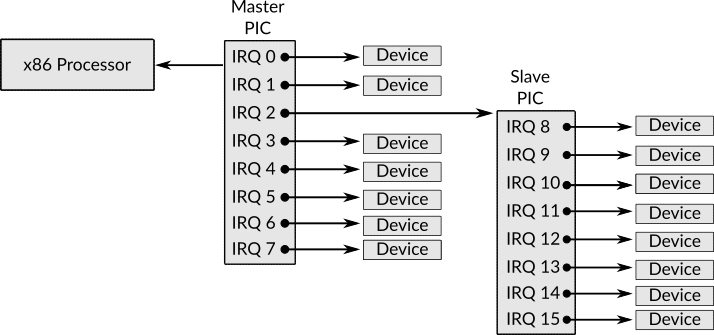
\includegraphics[width=0.50000\textwidth]{Figures/progenitor-ch/Fig21082021_0.png}
\caption{The Arrangement of Master and Slave PICs}\label{fig:21082021_0}
\end{figure}

Figure \ref{fig:21082021_0} shows this arrangement, as you can see, now,
there are \lstinline!15! slots in the whole system instead of only
\lstinline!8! slots. In the master PIC, the third slot
(\lstinline!IRQ2!) is connected to the slave PIC, that is, whatever
interrupt received by slave PIC from the devices that are attached to
it, will be sent to the master PIC through \lstinline!IRQ2!. All other
slots in both master (\lstinline!IRQ0! to \lstinline!IRQ7! but
\lstinline!IRQ2!) and slave PICs (\lstinline!IRQ8! to \lstinline!IRQ15!)
are connected to external devices. There is a standard which tells us
the device type that each \lstinline!IRQ! is dedicated to, for example,
\lstinline!IRQ0! is the interrupt which is received by a device known as
\emph{system timer} which is a device that sends an interrupt in each
unit of time which makes it extremely useful for multitasking
environment as we shall see later when we start discussing process
management, the following table shows the use of each \lstinline!IRQ!
\footnote{Source:
  \url{https://en.wikipedia.org/wiki/Interrupt_request_(PC_architecture)}}.

\begin{longtable}[]{@{}ll@{}}
\toprule
IRQ & Description\tabularnewline
\midrule
\endhead
0 & System Timer\tabularnewline
1 & Keyboard (PS/2 port)\tabularnewline
2 & Slave PIC\tabularnewline
3 & Serial Port 2 (COM)\tabularnewline
4 & Serial Port 1 (COM)\tabularnewline
5 & Parallel Port 3 or Sound Card\tabularnewline
6 & Floppy Disk Controller\tabularnewline
7 & Parallel Port 1\tabularnewline
8 & Real-time Clock\tabularnewline
9 & APCI\tabularnewline
10 & Available\tabularnewline
11 & Available\tabularnewline
12 & Mouse (PS/2 port)\tabularnewline
13 & Coprocessor\tabularnewline
14 & Primary ATA\tabularnewline
15 & Secondary ATA\tabularnewline
\bottomrule
\end{longtable}

After receiving an \lstinline!IRQ! from a device, PIC should send this
request to the processor, in this stage each \lstinline!IRQ! number is
mapped (or translated, if you prefer) to an interrupt number for the
processor, for example, \lstinline!IRQ0! will be sent to the processor
as interrupt number \lstinline!8!, \lstinline!IRQ1! will be mapped to
interrupt number \lstinline!9! and so on until \lstinline!IRQ7! which
will be mapped to interrupt number \lstinline!15d! (\lstinline!0Fh!),
while \lstinline!IRQ8! till \lstinline!IRQ15! will be mapped to
interrupts number from \lstinline!112d! (\lstinline!70h!) to
\lstinline!119d! (\lstinline!77h!).

In the real-mode, this mapping will be fine, but in protected-mode it is
going to cause conflicts between software and hardware interrupts, that
is, one interrupt number will be used by both software and hardware
which may causes some difficulties later in distinguishing the source of
this interrupt, is it from the software or hardware? For example, in
protected mode, interrupt number \lstinline!8! which is used for system
timer interrupt by PIC is also used by the processor when a software
error known as \emph{double fault} occurs. The good thing is that PIC is
\textbf{programmable}, which means that we can send commands to PIC and
tell it to change the default mapping (from \lstinline!IRQs! to
processor's interrupts number) to another mapping of our choice.

There are two well-known types of communicating with external devices by
the processor, we have already encountered one of them when we worked
with video memory which causes the processor to communicate with the
screen to write characters or draw pixels, this type of communication
from the processor to a devices is known as \emph{memory-mapped I/O}
communication, that is, the main memory is used to perform the
communication.

There is another type which is used by PIC and this type is known as
\emph{port-mapped I/O} communication. In this method, each device (that
uses this way) has \emph{ports}, each port has its own unique number and
job, for example, master PIC has two ports, the number of the first port
is \lstinline!20h! while the number of the second port is
\lstinline!21h!, the first port is used to send commands \footnote{Each
  device has its own set of commands.} to master PIC while the second
port is used to write data on it so the master PIC can read it. The same
is applicable to slave PIC with different port numbers, \lstinline!a0h!
and \lstinline!a1h! respectively. PIC has no explicit command to remap
\lstinline!IRQs!, instead, there is a command to initialize PIC, this
initialization consists of multiple steps and one of these steps it is
to set the required mapping. Now, we can present the skeleton of
\lstinline!setup_interrupts! as following.

\begin{lstlisting}
setup_interrupts:
    call remap_pic
    call load_idt
    
    ret
\end{lstlisting}

First, we are going to remap \lstinline!IRQs! to different interrupt
numbers by sending initialization command to both master and slave PICs,
then we are going to initialize and load \lstinline!IDT! and write the
necessary interrupts handlers which are also known as \emph{interrupt
service routines} (ISRs).

\subsection{Remapping PICs}\label{remapping-pics}

As we have said, we need to change the default mapping between
\lstinline!IRQs! and interrupt number of the processor to make sure that
there are no more than one source can emit a signal to one interrupt
number, this process is known as \emph{PIC remapping} which is simple to
perform. As we knew, PIC is a port-mapped I/O, and by using
\lstinline!out! instruction of x86 we can write something on a given
port number.

The \emph{initialization command} of PIC is represented by the number
\lstinline!11h!, which means writing this value on the command port of
PIC by using \lstinline!out! instruction is going to tell the PIC device
that we are going to initialize it. When we send this command to the PIC
through its own command port (\lstinline!20h! for master PIC and
\lstinline!a0h! for slave PIC), it is going to wait for us to write four
parameters on its data port (\lstinline!21h! for master PIC and
\lstinline!a1h! for slave PIC), the values of these parameters are
represented by numbers as we shall see in a moment.

The first parameter that should be provided to initialization command is
the new starting offset of \lstinline!IRQs!, for example, if the value
of this parameter is \lstinline!32d! for master PIC, that means
\lstinline!IRQ0! will be sent to the processor as interrupt number
\lstinline!32d! instead of \lstinline!8d! (as in default mapping),
\lstinline!IRQ1! will be sent to the processor as interrupt number
\lstinline!33d! and so on. The second parameter tells the PIC (that we
are initializing) in which of its slot the other PIC is connected. The
third parameter tells the PIC which mode we would like it to run on,
there are multiple modes for PIC devices, but the mode that we care
about and need to use is x86 mode. The fourth parameter tells the PIC
which \lstinline!IRQs! to enable and which to disable. Now, let's see
the code of \lstinline!remap_pic! routine which implements what we have
just described by setting the correct parameters to the initialization
command of both master and slave PICs.

\begin{lstlisting}
remap_pic:
    mov al, 11h
    
    send_init_cmd_to_pic_master:    
        out 0x20, al
        
    send_init_cmd_to_pic_slave:     
        out 0xa0, al
        
    ; ... ;
    
    make_irq_starts_from_intr_32_in_pic_master:     
        mov al, 32d
        out 0x21, al
    
    make_irq_starts_from_intr_40_in_pic_slave:
        mov al, 40d
        out 0xa1, al 
    
    ; ... ;
    
    tell_pic_master_where_pic_slave_is_connected:
        mov al, 04h
        out 0x21, al
    
    tell_pic_slave_where_pic_master_is_connected:
        mov al, 02h
        out 0xa1, al
    
    ; ... ;
    
    mov al, 01h
    
    tell_pic_master_the_arch_is_x86:
        out 0x21, al
    
    tell_pic_slave_the_arch_is_x86:
        out 0xa1, al
    
    ; ... ;
    
    mov al, 0h
    
    make_pic_master_enables_all_irqs:
        out 0x21, al
    
    make_pic_slave_enables_all_irqs:
        out 0xa1, al
    
    ; ... ;
    
    ret
\end{lstlisting}

Note that the labels here are optional, I've added them for the sake of
readability, you can get rid of them if you want. As you can see, the
command and data port for both master and slave PICs are used to send
initialize command and the parameters. The instruction \lstinline!out!
can only take the register \lstinline!ax! as second operand and due to
that, the number that represent the command or the data that we would
like to send are always set to \lstinline!al! first which is used later
as the second operand of \lstinline!out!. Also, it should be obvious
that the first operand of \lstinline!out! is the port number, while the
second operand is the value that we would like to send.

\begin{figure}
\centering
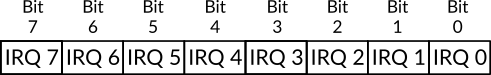
\includegraphics[width=0.50000\textwidth]{Figures/progenitor-ch/Fig27082021_0.png}
\caption{Master PIC's Data Format to Set The Place of Slave
PIC}\label{fig:27082021_0}
\end{figure}

You may ask, why the value is \lstinline!4! is used in the label
\lstinline!tell_pic_master_where_pic_slave_is_connected! \footnote{I
  just realized that this is a really long name! Sorry, sometimes I
  become a readability freak!} instead of \lstinline!2! since we said
earlier that the salve PIC is connected to master PIC through
\lstinline!IRQ2!. The reason of that is the format of the data that
should be sent to master PIC in order to tell it the place where slave
PIC is attached to. This format is shown in figure \ref{fig:27082021_0}
which shows that the size of the data is \lstinline!1! byte and each
\lstinline!IRQ! is represented by one bit, that is, each bit is used as
a flag to indicate which \lstinline!IRQ! we would like to use.

\begin{figure}
\centering
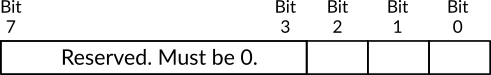
\includegraphics[width=0.50000\textwidth]{Figures/progenitor-ch/Fig27082021_1.png}
\caption{Slave PIC's Data Format to Set The Place of Master
PIC}\label{fig:27082021_1}
\end{figure}

In our case, slave PIC is connected to master PIC through
\lstinline!IRQ2! which is represented by bit \lstinline!2!, which means
the value of this bit should be \lstinline!1! and all other bits should
be \lstinline!0!, this gives us the binary sequence
\lstinline!0000 0100! which is \lstinline!4d!. Assume that the slave PIC
is connect to master PIC through \lstinline!IRQ7!, then the binary
sequence will be \lstinline!1000 0000!, which is \lstinline!128d!. For
the slave PIC, the format is shown in figure \ref{fig:27082021_1} and as
you can see, only bits \lstinline!0! to \lstinline!2! can be used while
the others should be \lstinline!0!. By using these three bits we can
represent the number \lstinline!8! at most, the normal way of
representing the numbers can be used here and for that the value
\lstinline!2! is passed to slave PIC to tell it that it is connected to
master PIC through \lstinline!IRQ2! in the label
\lstinline!tell_pic_slave_where_pic_master_is_connected!.

\subsection{Writing ISRs and Loading
IDT}\label{writing-isrs-and-loading-idt}

Right now, everything is ready to write the code of loading
\lstinline!IDT! and \lstinline!ISR!s. The first one is too simple and
similar to the code of loading the \lstinline!GDT! table, the following
is the code of \lstinline!load_idt! routine.

\begin{lstlisting}
load_idt:
    lidt [idtr - start]
    ret
\end{lstlisting}

As you can see, nothing is new here. The instruction \lstinline!lidt! is
used to load the content of the register \lstinline!idtr! by using the
same way that we have already used in the previous routine
\lstinline!load_gdt!. Now, for the sake of organizing, I'm going to
dedicate a new file for the related stuff of \lstinline!IDT! and
\lstinline!ISR!s and this file will be called \lstinline!idt.asm!. In
the end of \lstinline!starter.asm! the following line should be added
\lstinline!%include "idt.asm"!, exactly as we did with
\lstinline!gdt.asm!.

At least, we need to define \lstinline!49! \lstinline!ISR!s since the
interrupts from \lstinline!0! to \lstinline!31! are used by the
processor to indicate that some error happened in the system. In fact,
interrupts \lstinline!22! to \lstinline!31! are reserved and has no use
for us, but we need to fill their entries in the \lstinline!IDT! table
to be able to use the interrupts starting from \lstinline!32!. While the
interrupts \lstinline!32! to \lstinline!48! are now used by PIC after
the remapping for hardware interrupts (\lstinline!IRQs!). Hence, we need
to fill the entries of all of these interrupts in the \lstinline!IDT! to
make sure that our kernel runs correctly. Right now, we are going to use
the same skeleton for the \lstinline!ISRs! that we are going to define,
let's start with \lstinline!isr_0! which is the name of the routine that
handles interrupt \lstinline!0!. Starting from here, the code that are
presented should be in the file \lstinline!idt.asm! unless otherwise is
mentioned explicitly.

\begin{lstlisting}
isr_0:
    cli
    push 0
    jmp isr_basic
\end{lstlisting}

The code here is too simple, we first make sure that interrupts are
disabled by using the instruction \lstinline!cli!; in the time that we
are handling an interrupt, we don't want another interrupt to occur, it
will be more obvious why this is important when we start to implement
process management in 539kernel.

After disabling the interrupts, we push to the stack the value
\lstinline!0! which is the number of the current interrupt, this pushed
value can be used later by a C function that we are going to call as a
parameter \footnote{That's possible due to the calling convention as we
  have discussed earlier in the previous chapter \ref{ch-x86}.}, in this
way, we can have just one C function that works as an interrupt handler
which receives a parameter that holds the interrupt number which should
be handled. After pushing the interrupt number, the routine is going to
jump to the label \lstinline!isr_basic! which contains the basic code of
all \lstinline!ISRs! that we are going to define.

Now, for all other \lstinline!ISRs! that are related to the processor,
that is, from interrupt \lstinline!1! to \lstinline!31! we are going to
use the exact same code, only two things should be changed, the name of
the routine should indicate the interrupt number, for example
\lstinline!isr_1! for interrupt \lstinline!1!, \lstinline!isr_2! for
\lstinline!2! and so on, the second change is the pushed value. I'm not
going to show you all \lstinline!31! \lstinline!ISR!s in here since they
need a lot of space, but you can always refer to 539kernel source code
if the matter isn't clear for you and the following is an example of
\lstinline!ISRs! \lstinline!1!, \lstinline!2! and \lstinline!3!. The
label \lstinline!isr_basic! will be defined later on.

\begin{lstlisting}
isr_1:
    cli
    push 1
    jmp isr_basic
    
isr_2:
    cli
    push 2
    jmp isr_basic
    
isr_3:
    cli
    push 3
    jmp isr_basic
\end{lstlisting}

The second set of \lstinline!ISR!s is the one that handles the
\lstinline!IRQ!s and the interrupt numbers here, as we mentioned
earlier, starts from \lstinline!32! to \lstinline!48!. The following is
an example of one of them which is \lstinline!isr_32!.

\begin{lstlisting}
isr_32:
    cli
    push 32
    jmp irq_basic
\end{lstlisting}

It's exactly the same code as the \lstinline!ISR!s before
\lstinline!32!, the only difference is the label that will the routine
jumps to. In the current case it is \lstinline!irq_basic!, which is the
basic code for all interrupts that handles the \lstinline!IRQs!, hence,
\lstinline!isr_33! till \lstinline!isr_48! has the same code as
\lstinline!isr_32! but with changing the pushed value. The following is
the code of \lstinline!isr_basic!.

\begin{lstlisting}
isr_basic:
    call interrupt_handler
    
    pop eax
    
    sti
    iret
\end{lstlisting}

Simply, \lstinline!isr_basic! calls a function known as
\lstinline!interrupt_handler! which is a C function that is going to be
in the main kernel code, to make \lstinline!NASM! able to know that this
function is defined elsewhere than the assembly code, the line
\lstinline!extern interrupt_handler! should be added before
\lstinline!start! routine in \lstinline!starter.asm!, exactly as we did
with the function \lstinline!kernel_main!.

After the function \lstinline!interrupt_handler! returns, the stack of
the current \lstinline!ISR! is cleaned by eliminating the value that we
have pushed which represents the number of the current interrupt, this
is performed by using \lstinline!pop! instruction which requires an
operand to store the popped value on it and for no reason I've chosen
\lstinline!eax!. This is a simplest way of cleaning the stack's frame,
another well known way is \lstinline!add esp, 4! where the second
operand is the size of all data that we have pushed on the frame and we
would like to eliminate before return, in our case, the size of the
number that we have pushed is \lstinline!4! bytes. As you can see, the
latter method of cleaning the stack is more preferred since no place to
store the popped value is needed and most probably you are going to
encounter this method in the real codes much more. For the sake of
simplicity, I'm going to keep the earlier method in the current case
unless the other is needed.

Finally, the \lstinline!ISR! re-enables the interrupts with the
instruction \lstinline!sti! and returns by using the instruction
\lstinline!iret! instead of the normal \lstinline!ret! that we have used
before, the former one is the one that should be used by interrupt
handlers to return. The following is the code of \lstinline!irq_basic!.

\begin{lstlisting}
irq_basic:
    call interrupt_handler
    
    mov al, 0x20
    out 0x20, al
    
    cmp byte [esp], 40d
    jnge irq_basic_end
    
    mov al, 0xa0
    out 0x20, al
    
    irq_basic_end:
        pop eax
        
        sti
        iret
\end{lstlisting}

The fundamental functionality of \lstinline!irq_basic! is same as
\lstinline!isr_basic!, it calls the C function
\lstinline!interrupt_handler! and in the end it cleans the stack and
returns (in label \lstinline!irq_basic_end!), the question now, what is
this additional code between calling the C function and returning? As
you know, \lstinline!IRQs! come from one of the PICs of the system, and
this \lstinline!PCI! requires to be told that the \lstinline!IRQ! it
sent has been handled, to do that the PIC command known as \emph{end of
interrupt} (\lstinline!EOI!) should be used and that's what the code
does.

The command \lstinline!EOI! should be sent to the master PIC after
handling all \lstinline!IRQs! (the ones that belong to the master and
also the slave), but for the slave \lstinline!PIC! this command should
be sent only after the \lstinline!IRQs! of slave PIC are handled, that
is, interrupt number \lstinline!40! till \lstinline!48!. So, after
returning from the C function \lstinline!interrupt_handler!, the command
\lstinline!EOI! is sent directly to the mater PIC. As you can see, we
write the value \lstinline!20h! to the port \lstinline!20h!, the first
value represents that \lstinline!EOI! command, while the second value
represents the command port of master PIC as we learned earlier. After
that, the interrupt number, that we have pushed on the stack in the
beginning of the \lstinline!ISR!, is used to check if the interrupt that
we have handled is greater than or equal \lstinline!40d!, if this is not
the case, a jump is performed to \lstinline!irq_basic_end!, otherwise,
\lstinline!EOI! command is sent to the slave PIC through its command
port \lstinline!a0h!.

Now, we are ready to define the \lstinline!IDT! table, to not take too
much space I will show only the first three entries, but the full table
should have \lstinline!49! entries, all of them with the same exact
fields and the only difference is the label name of the \lstinline!ISR!
\footnote{The values of the properties here are used from Basekernel
  project (\url{https://github.com/dthain/basekernel}).}.

\begin{lstlisting}
idt:
    dw isr_0, 8, 0x8e00, 0x0000
    dw isr_1, 8, 0x8e00, 0x0000
    dw isr_2, 8, 0x8e00, 0x0000
\end{lstlisting}

The meaning of the values of the fields are summarized in the following
table.

\begin{longtable}[]{@{}llllll@{}}
\toprule
\begin{minipage}[b]{0.15\columnwidth}\raggedright\strut
Handler's Name\strut
\end{minipage} & \begin{minipage}[b]{0.18\columnwidth}\raggedright\strut
Segment Selector\strut
\end{minipage} & \begin{minipage}[b]{0.09\columnwidth}\raggedright\strut
Present\strut
\end{minipage} & \begin{minipage}[b]{0.16\columnwidth}\raggedright\strut
Privilege Level\strut
\end{minipage} & \begin{minipage}[b]{0.16\columnwidth}\raggedright\strut
Descriptor Size\strut
\end{minipage} & \begin{minipage}[b]{0.11\columnwidth}\raggedright\strut
Gate Type\strut
\end{minipage}\tabularnewline
\midrule
\endhead
\begin{minipage}[t]{0.15\columnwidth}\raggedright\strut
isr\_0\strut
\end{minipage} & \begin{minipage}[t]{0.18\columnwidth}\raggedright\strut
8 (Kernel's Code)\strut
\end{minipage} & \begin{minipage}[t]{0.09\columnwidth}\raggedright\strut
Yes\strut
\end{minipage} & \begin{minipage}[t]{0.16\columnwidth}\raggedright\strut
0\strut
\end{minipage} & \begin{minipage}[t]{0.16\columnwidth}\raggedright\strut
32-bit\strut
\end{minipage} & \begin{minipage}[t]{0.11\columnwidth}\raggedright\strut
Interrupt\strut
\end{minipage}\tabularnewline
\begin{minipage}[t]{0.15\columnwidth}\raggedright\strut
isr\_1\strut
\end{minipage} & \begin{minipage}[t]{0.18\columnwidth}\raggedright\strut
8 (Kernel's Code)\strut
\end{minipage} & \begin{minipage}[t]{0.09\columnwidth}\raggedright\strut
Yes\strut
\end{minipage} & \begin{minipage}[t]{0.16\columnwidth}\raggedright\strut
0\strut
\end{minipage} & \begin{minipage}[t]{0.16\columnwidth}\raggedright\strut
32-bit\strut
\end{minipage} & \begin{minipage}[t]{0.11\columnwidth}\raggedright\strut
Interrupt\strut
\end{minipage}\tabularnewline
\begin{minipage}[t]{0.15\columnwidth}\raggedright\strut
isr\_2\strut
\end{minipage} & \begin{minipage}[t]{0.18\columnwidth}\raggedright\strut
8 (Kernel's Code)\strut
\end{minipage} & \begin{minipage}[t]{0.09\columnwidth}\raggedright\strut
Yes\strut
\end{minipage} & \begin{minipage}[t]{0.16\columnwidth}\raggedright\strut
0\strut
\end{minipage} & \begin{minipage}[t]{0.16\columnwidth}\raggedright\strut
32-bit\strut
\end{minipage} & \begin{minipage}[t]{0.11\columnwidth}\raggedright\strut
Interrupt\strut
\end{minipage}\tabularnewline
\bottomrule
\end{longtable}

As in \lstinline!GDT! table, I've written a Python script that let you
manipulate the properties of descriptors by getting a human readable
input, the code of the script is the following.

\begin{lstlisting}[language=Python]
import json;

def generateIDTAsWords( idtAsJSON, nasmFormat = False ):
    idt = json.loads( idtAsJSON );
    idtAsWords = '';
    
    for entry in idt:
        if nasmFormat:
            idtAsWords += 'dw ';
        
        # ... #
        
        present = ( 1 if entry[ 'present' ] else 0 ) << 7;
        dpl = entry[ 'dpl' ] << 6;
        size = ( 1 if entry[ 'gate_descriptor_size' ] == '32-bit' else 0 ) << 3;
        gateType = ( 0 if entry[ 'interrupt_gate' ] else 1 );
        
        byteFive = present | dpl | ( 0 << 11 ) | size | ( 1 << 2 ) | ( 1 << 1 ) | gateType;
        
        wordThree = '0x' + format( byteFive, 'x' ).zfill( 2 ) + '00';
        
        # ... #
        
        idtAsWords += entry[ 'isr_routine_name' ] + ', ' + str( entry[ 'isr_segment_selector' ] ) + ', ' + wordThree + ', 0x0000'  + '\n';
        
    return idtAsWords;
\end{lstlisting}

The following is an example of using \lstinline!generateIDTAsWords!.

\begin{lstlisting}[language=Python]
idt = '''
[
    {   "isr_routine_name": "isr_0", "isr_segment_selector": 8, "present": true, "dpl": 0, "gate_descriptor_size": "32-bit", "interrupt_gate": true },
    {   "isr_routine_name": "isr_1", "isr_segment_selector": 8, "present": true, "dpl": 0, "gate_descriptor_size": "32-bit", "interrupt_gate": true }
]
''';

print( generateIDTAsWords( idt, True ) );
\end{lstlisting}

After defining the entries of \lstinline!IDT!, we can define the label
\lstinline!idtr! which will be the value that we will load in the
special register \lstinline!idtr!.

\begin{lstlisting}
idtr:
    idt_size_in_bytes   :   dw idtr - idt
    idt_base_address    :   dd idt
\end{lstlisting}

It should be easy to you now to know why \lstinline!idtr - idt! gives us
the size of \lstinline!IDT! in bytes. Also, you should know that if the
label \lstinline!idtr! is not right below the label \lstinline!idt! this
will not work. I've used this method instead of hardcoding the size of
the table \lstinline!8 * 49 = 392! in the code to make sure that I don't
forget to change the size field when I add a new entry in
\lstinline!IDT!, you are free to hardcode the size as we did in
\lstinline!gdtr! if you like to. Finally, the C function
\lstinline!interrupt_handler! can be defined in the end of
\lstinline!main.c! as following.

\begin{lstlisting}[language=C]
void interrupt_handler( int interrupt_number )
{
    println();
    print( "Interrupt Received " );
    printi( interrupt_number );
}
\end{lstlisting}

It simply receives the interrupt number as a parameter, as you have
expected, and prints this number in an appealing way.

And now we have got the progenitor of 539kernel! Compiling and running
this code is going to print the messages
\lstinline"Welcome to 539kernel!" then
\lstinline!We are now in Protected-mode! then \lstinline!539! and
finally, our first interrupt will be received and the message
\lstinline!Interrupt Received 32! will be printed on the screen, this
interrupt will not be received just once since it is the interrupt of
the system timer the kernel will keep receiving it and prints the same
message every given unit of time. We will use the system timer later
when we start discussing the scheduling of processes in chapter
\ref{ch-progenitor}.

\section{Quick View of the Changes of
Makefile}\label{quick-view-of-the-changes-of-makefile}

As you may have noticed, the \lstinline!Makefile! of the progenitor
version of 539kernel has some different aspects than the one that we
have used in the bootloader version of 539kernel. The first difference
is the way that we assemble \lstinline!starter.asm!, as you can see,
unlike \lstinline!bootstrap.asm!, the output of the process of
assembling the starter is an \lstinline!ELF32! binary file instead of
flat binary file. As you know, the code of the starter is related to the
C code of 539kernel, that is, there are C functions that are called in
the starter code. To make the starter able to reach this C code
correctly, the binary output of both \lstinline!starter.asm! and
\lstinline!main.c! should be linked. It is the responsibility of the
linker to generate a final binary file that understands what the starter
mean when it calls the C function \lstinline!interrupt_handler! for
example. If the linking process between the two files is not performed,
the starter will never know where is the code of
\lstinline!interrupt_handler! or \lstinline!kernel_main!.

To link two binary files, they should have the same format and this
format makes it possible to link the files that generated by using it.
GCC generates \lstinline!ELF! binary files by default, so, when we
assemble \lstinline!starter.asm! we tell \lstinline!NASM! to generate
and \lstinline!ELF! file. After that the output binary files (AKA:
object files) of both \lstinline!starter.asm! and \lstinline!main.c! are
linked by using the command \lstinline!ld!, we tell the linker that we
are linking \lstinline!ELF! object files, the order of the files that we
pass to the linker to link is important, as you can see
\lstinline!starter.o! is passed before \lstinline!kernel.elf!, which
makes the linker puts the code of the starter before the code of the
main kernel in the final output \lstinline!ELF! binary file
\lstinline!539kernel.elf!. Because \lstinline!ELF! is not understandable
by the machine unless some code interprets it, we convert it to a flat
binary file by using the command \lstinline!objcopy!, in this way, the
bootloader can load the kernel without the need of dealing with the
details of \lstinline!ELF! format.

Also, you can see that the final image of the kernel
\lstinline!kernel.img! is generated by writing the content of bootloader
first, then the kernel and then the image is fill with around
\lstinline!1MB! of zeros, while this step isn't necessary for QEMU, but
if you decide to use Bochs instead, such a step is required. While we
are going to stick with the former one right now, the latter one, in my
humble opinion, has better debugging tools.

Another important aspect of the new \lstinline!Makefile! is the flags
that are passed to GCC, we need to be careful with these flags and pass
the correct ones to make sure that GCC compiles our kernel correctly
since GCC compiles user-space applications by default. The flag
\lstinline!-Wall! tells GCC to show us the warnings on our code. The
flag \lstinline!-m32! makes GCC generate \lstinline!32-bit! code. The
flag \lstinline!-c! stops the linker from running by default since we
are going to run it later manually with specific options as you have
seen. The flag \lstinline!-ffreestanding! indicates that we are
compiling a code that the standard library of C is not available for it
and the \lstinline!main! function is not necessary for it. Both flags
\lstinline!-fno-asynchronous-unwind-tables! and \lstinline!-fno-pie! are
used to eliminate some extra code that is generated by the GCC to handle
some situations that are related to user-space code. This is a quick
review of the functionality of the flags and you can always refer to the
official documentation of GCC for more details.

\section{A Traditionalist Implementer or a
Kernelist?}\label{a-traditionalist-implementer-or-a-kernelist}

Most probably you are objecting, ``\textbf{kernelist} is not even a
word!'' I know, even my poor spell checker is shocked! Just bear with me
a little bit and let me show you what I mean by the term
\emph{kernelist}.

In our journey of creating an operating system kernel we may ask
ourselves, what is our role exactly? There are two possible roles that I
would like to focus on, the first one is being a traditionalist
implementer (for short: traditionalist). What I mean by the
traditionalist is the one who writes the code of the kernel without
focusing too much on the design of the kernel and the philosophical
questions about that kernel, examples of these questions are ``What is
the problem that the kernel will solve?'', ``How to design its
architecture to accomplish its goal'' and so on, also the traditionalist
tends to implement already well-known solutions that have been used many
years with no or little changes. The kernelist, on the other hand, is
the person who takes care of the questions about kernel's design and the
new solutions for the problems and tries to answer these questions and
presents a suitable kernel's design and solutions for specific problems.
For example, writing a Unix-like kernel is the job of traditionalist,
since the architecture of Unix is already designed by kernelists to
solve specific problems.

Our goal from this book is to \textbf{learn} how to write an operating
system kernel with a traditional design and no new ideas, so, we are
taking the role of a traditionalist, the design of 539kernel is too
simple and it solves no specific problem in a novel way, instead it uses
the concepts that are already there and used by many operating systems
as you will see in the next chapters, also it doesn't focus on some new
problem to solve nor a new solution for an old problem, this makes
539kernel a working kernel that solves the same problems that other
kernels solve by using the same methods that other kernels use, the
advantage of this design is making 539kernel easy to implement which
means it is a good starting point to learn about operating system
kernels and that's the goal of this book.

The natural question for someone, who would like to continue in the
journey of operating system kernels, to ask herself after implementing a
basic kernel, ``What's next?'' and here where a kernelist is born! In
fact, there are many real world problems in computing that need to be
solved, also, there are many innovative ideas that need to be created,
furthermore, there are many good ideas that have been presented by
someone else but need to be realized in the real world systems, a lot of
aforementioned can be found in the scientific papers \footnote{In fact,
  I've started a project that generalize this thought and I called it
  \lstinline!ResearchCoders!. If you are interested in finding and
  implementing new ideas that solve real-world problems you may would
  like to check the website of the project
  (\url{https://researchcoders.dev})}.

The kernelist doesn't necessarily innovate new solutions by himself, but
he can use modern solutions that have been proposed by other kernelist
to implement and design a kernel with modern innovative and useful ideas
instead of reimplementing the traditional solutions that have been with
us for \lstinline!60! years over and over again.

After reading this book to learn about creating a kernel and you would
like to continue the journey, I encourage you to consider the role of
kernelist. Using what you have learned to solve real-world problem is a
good idea, and the world needs this kind of orientation. Although this
is a book of traditionalist more that a kernelist, I've dedicated
chapter \ref{ch-wthat-is-next} for those who would like to, at least,
take a look on being kernelist.
